%
% 
%
% Copyright (C) 1997-2002 by Dimitri van Heesch.
%
% Permission to use, copy, modify, and distribute this software and its
% documentation under the terms of the GNU General Public License is hereby 
% granted. No representations are made about the suitability of this software 
% for any purpose. It is provided "as is" without express or implied warranty.
% See the GNU General Public License for more details.
%
% Documents produced by Doxygen are derivative works derived from the
% input used in their production; they are not affected by this license.

\documentclass[a4paper]{article}
\usepackage{a4wide}
\usepackage{makeidx}
\usepackage{fancyhdr}
\usepackage{float}
\usepackage{graphicx}
\usepackage{epsf}
\usepackage{doxygen}
\usepackage{multicol}
\usepackage{times}
\usepackage{alltt}
\usepackage[pdftex,
            pagebackref=true,
            colorlinks=true,
            linkcolor=blue
           ]{hyperref}
\makeindex
\setcounter{tocdepth}{1}
\setlength{\footrulewidth}{0.4pt}
\begin{document}
\begin{titlepage}
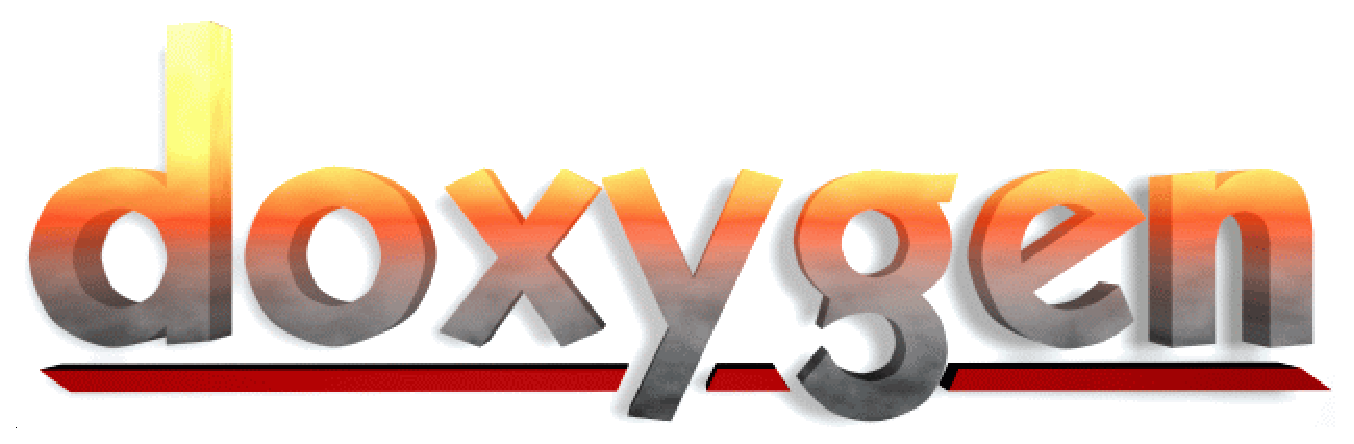
\includegraphics[width=\textwidth]{doxygen_logo}
\begin{center}
Manual for version $VERSION\\[2ex]
Written by Dimitri van Heesch\\[2ex]
\copyright 1997-2002
\end{center}
\end{titlepage}
\clearemptydoublepage
\tableofcontents
\clearemptydoublepage
\pagenumbering{arabic}
\include{index}
\part{User Manual}
\input{install}
\input{starting}
\input{docblocks}
\input{lists}
\input{grouping}
\input{formulas}
PROJECT_NAME       = "Diagrams"
OUTPUT_DIRECTORY   = ../html/examples/diagrams
HAVE_DOT           = YES
EXTRACT_ALL        = YES
GENERATE_LATEX     = YES
GENERATE_MAN       = NO
GENERATE_RTF       = NO
CASE_SENSE_NAMES = NO
ENABLE_PREPROCESSING       = YES
INPUT              = .
STRIP_CODE_COMMENTS = NO
FILE_PATTERNS      = diagrams_*.h
QUIET              = YES
JAVADOC_AUTOBRIEF = YES
SEARCHENGINE     = NO
COMPACT_LATEX = YES
LATEX_HIDE_INDICES     = YES

\input{preprocessing}
\input{external}
\input{faq}
\input{trouble}
\part{Reference Manual}
\input{features}
\input{history}
\input{doxygen_usage}
\input{doxytag_usage}
\input{doxysearch_usage}
\input{doxywizard_usage}
\input{installdox_usage}
\input{output}
PROJECT_NAME     = "Automatic link generation"
OUTPUT_DIRECTORY = autolink
GENERATE_LATEX   = NO
GENERATE_MAN     = NO
GENERATE_RTF     = NO
CASE_SENSE_NAMES = NO
INPUT            = autolink.cpp
QUIET            = YES
JAVADOC_AUTOBRIEF = YES
SEARCHENGINE     = NO

\input{config}
\input{commands}
\input{htmlcmds}
\part{Developers Manual}
\input{arch}
\input{langhowto}
\printindex
\end{document}
